\documentclass[aspectratio=169]{beamer}
\usepackage{iftex}
\ifPDFTeX
  \usepackage[T1]{fontenc}
  \usepackage[utf8]{inputenc}
  \usepackage{lmodern}
\else
  \usepackage{fontspec}
\fi
\usepackage{lipsum}
\usepackage{tikz}
\usetheme{Madrid}
\title{A 40-slide deck for the compile benchmark}
\author{Purplelink LLC}
\date{October 2026}
\begin{document}
\begin{frame}\titlepage\end{frame}
\begin{frame}{Outline}Edit marker: alpha.
\tableofcontents\end{frame}
\section{Slides}
\begin{frame}{Slide 1: synthetic topic}
\begin{itemize}
  \item \lipsum[2][1]
  \item \lipsum[3][2]
\end{itemize}
\begin{center}
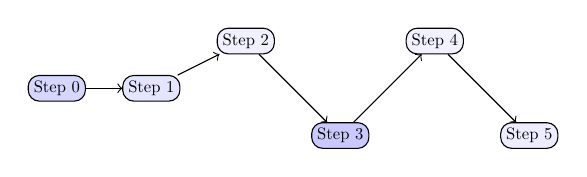
\begin{tikzpicture}[scale=0.6, transform shape]
  \node[draw,rounded corners,fill=blue!16] (n0) at (0.0,0) {Step 0};
  \node[draw,rounded corners,fill=blue!10] (n1) at (2.0,0) {Step 1};
  \node[draw,rounded corners,fill=blue!6] (n2) at (4.0,1) {Step 2};
  \node[draw,rounded corners,fill=blue!21] (n3) at (6.0,-1) {Step 3};
  \node[draw,rounded corners,fill=blue!5] (n4) at (8.0,1) {Step 4};
  \node[draw,rounded corners,fill=blue!7] (n5) at (10.0,-1) {Step 5};
  \draw[->] (n0) -- (n1);
  \draw[->] (n1) -- (n2);
  \draw[->] (n2) -- (n3);
  \draw[->] (n3) -- (n4);
  \draw[->] (n4) -- (n5);
\end{tikzpicture}
\end{center}
\end{frame}
\begin{frame}{Slide 2: synthetic topic}
\begin{itemize}
  \item \lipsum[3][1]
  \item \lipsum[4][2]
\end{itemize}
\begin{center}
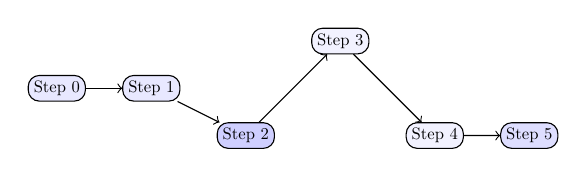
\begin{tikzpicture}[scale=0.6, transform shape]
  \node[draw,rounded corners,fill=blue!9] (n0) at (0.0,0) {Step 0};
  \node[draw,rounded corners,fill=blue!9] (n1) at (2.0,0) {Step 1};
  \node[draw,rounded corners,fill=blue!19] (n2) at (4.0,-1) {Step 2};
  \node[draw,rounded corners,fill=blue!5] (n3) at (6.0,1) {Step 3};
  \node[draw,rounded corners,fill=blue!5] (n4) at (8.0,-1) {Step 4};
  \node[draw,rounded corners,fill=blue!13] (n5) at (10.0,-1) {Step 5};
  \draw[->] (n0) -- (n1);
  \draw[->] (n1) -- (n2);
  \draw[->] (n2) -- (n3);
  \draw[->] (n3) -- (n4);
  \draw[->] (n4) -- (n5);
\end{tikzpicture}
\end{center}
\end{frame}
\begin{frame}{Slide 3: synthetic topic}
\begin{itemize}
  \item \lipsum[4][1]
  \item \lipsum[5][2]
\end{itemize}
\begin{center}
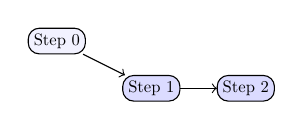
\begin{tikzpicture}[scale=0.6, transform shape]
  \node[draw,rounded corners,fill=blue!5] (n0) at (0.0,1) {Step 0};
  \node[draw,rounded corners,fill=blue!14] (n1) at (2.0,0) {Step 1};
  \node[draw,rounded corners,fill=blue!14] (n2) at (4.0,0) {Step 2};
  \draw[->] (n0) -- (n1);
  \draw[->] (n1) -- (n2);
\end{tikzpicture}
\end{center}
\end{frame}
\begin{frame}{Slide 4: synthetic topic}
\begin{itemize}
  \item \lipsum[5][1]
  \item \lipsum[6][2]
\end{itemize}
\begin{center}
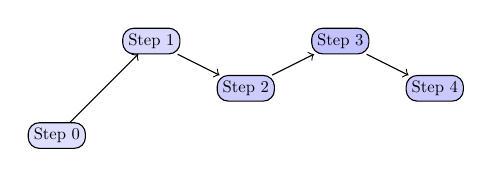
\begin{tikzpicture}[scale=0.6, transform shape]
  \node[draw,rounded corners,fill=blue!13] (n0) at (0.0,-1) {Step 0};
  \node[draw,rounded corners,fill=blue!15] (n1) at (2.0,1) {Step 1};
  \node[draw,rounded corners,fill=blue!20] (n2) at (4.0,0) {Step 2};
  \node[draw,rounded corners,fill=blue!24] (n3) at (6.0,1) {Step 3};
  \node[draw,rounded corners,fill=blue!21] (n4) at (8.0,0) {Step 4};
  \draw[->] (n0) -- (n1);
  \draw[->] (n1) -- (n2);
  \draw[->] (n2) -- (n3);
  \draw[->] (n3) -- (n4);
\end{tikzpicture}
\end{center}
\end{frame}
\begin{frame}{Slide 5: synthetic topic}
\begin{itemize}
  \item \lipsum[6][1]
  \item \lipsum[7][2]
\end{itemize}
\begin{center}
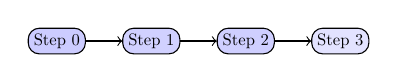
\begin{tikzpicture}[scale=0.6, transform shape]
  \node[draw,rounded corners,fill=blue!20] (n0) at (0.0,0) {Step 0};
  \node[draw,rounded corners,fill=blue!18] (n1) at (2.0,0) {Step 1};
  \node[draw,rounded corners,fill=blue!19] (n2) at (4.0,0) {Step 2};
  \node[draw,rounded corners,fill=blue!11] (n3) at (6.0,0) {Step 3};
  \draw[->] (n0) -- (n1);
  \draw[->] (n1) -- (n2);
  \draw[->] (n2) -- (n3);
\end{tikzpicture}
\end{center}
\end{frame}
\begin{frame}{Slide 6: synthetic topic}
\begin{itemize}
  \item \lipsum[7][1]
  \item \lipsum[8][2]
\end{itemize}
\begin{center}
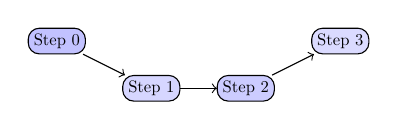
\begin{tikzpicture}[scale=0.6, transform shape]
  \node[draw,rounded corners,fill=blue!24] (n0) at (0.0,1) {Step 0};
  \node[draw,rounded corners,fill=blue!16] (n1) at (2.0,0) {Step 1};
  \node[draw,rounded corners,fill=blue!20] (n2) at (4.0,0) {Step 2};
  \node[draw,rounded corners,fill=blue!14] (n3) at (6.0,1) {Step 3};
  \draw[->] (n0) -- (n1);
  \draw[->] (n1) -- (n2);
  \draw[->] (n2) -- (n3);
\end{tikzpicture}
\end{center}
\end{frame}
\begin{frame}{Slide 7: synthetic topic}
\begin{itemize}
  \item \lipsum[8][1]
  \item \lipsum[9][2]
\end{itemize}
\begin{center}
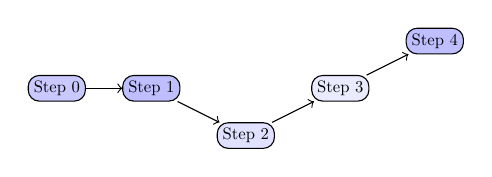
\begin{tikzpicture}[scale=0.6, transform shape]
  \node[draw,rounded corners,fill=blue!21] (n0) at (0.0,0) {Step 0};
  \node[draw,rounded corners,fill=blue!25] (n1) at (2.0,0) {Step 1};
  \node[draw,rounded corners,fill=blue!12] (n2) at (4.0,-1) {Step 2};
  \node[draw,rounded corners,fill=blue!8] (n3) at (6.0,0) {Step 3};
  \node[draw,rounded corners,fill=blue!25] (n4) at (8.0,1) {Step 4};
  \draw[->] (n0) -- (n1);
  \draw[->] (n1) -- (n2);
  \draw[->] (n2) -- (n3);
  \draw[->] (n3) -- (n4);
\end{tikzpicture}
\end{center}
\end{frame}
\begin{frame}{Slide 8: synthetic topic}
\begin{itemize}
  \item \lipsum[9][1]
  \item \lipsum[10][2]
\end{itemize}
\begin{center}
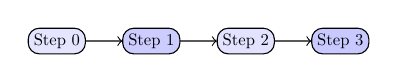
\begin{tikzpicture}[scale=0.6, transform shape]
  \node[draw,rounded corners,fill=blue!10] (n0) at (0.0,-1) {Step 0};
  \node[draw,rounded corners,fill=blue!20] (n1) at (2.0,-1) {Step 1};
  \node[draw,rounded corners,fill=blue!11] (n2) at (4.0,-1) {Step 2};
  \node[draw,rounded corners,fill=blue!21] (n3) at (6.0,-1) {Step 3};
  \draw[->] (n0) -- (n1);
  \draw[->] (n1) -- (n2);
  \draw[->] (n2) -- (n3);
\end{tikzpicture}
\end{center}
\end{frame}
\begin{frame}{Slide 9: synthetic topic}
\begin{itemize}
  \item \lipsum[10][1]
  \item \lipsum[11][2]
\end{itemize}
\begin{center}
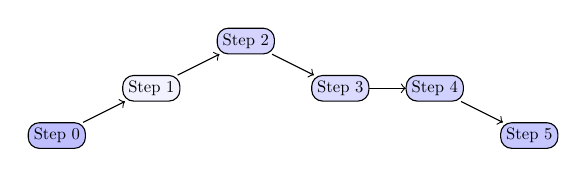
\begin{tikzpicture}[scale=0.6, transform shape]
  \node[draw,rounded corners,fill=blue!25] (n0) at (0.0,-1) {Step 0};
  \node[draw,rounded corners,fill=blue!5] (n1) at (2.0,0) {Step 1};
  \node[draw,rounded corners,fill=blue!17] (n2) at (4.0,1) {Step 2};
  \node[draw,rounded corners,fill=blue!14] (n3) at (6.0,0) {Step 3};
  \node[draw,rounded corners,fill=blue!18] (n4) at (8.0,0) {Step 4};
  \node[draw,rounded corners,fill=blue!22] (n5) at (10.0,-1) {Step 5};
  \draw[->] (n0) -- (n1);
  \draw[->] (n1) -- (n2);
  \draw[->] (n2) -- (n3);
  \draw[->] (n3) -- (n4);
  \draw[->] (n4) -- (n5);
\end{tikzpicture}
\end{center}
\end{frame}
\begin{frame}{Slide 10: synthetic topic}
\begin{itemize}
  \item \lipsum[11][1]
  \item \lipsum[12][2]
\end{itemize}
\begin{center}
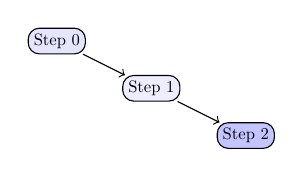
\begin{tikzpicture}[scale=0.6, transform shape]
  \node[draw,rounded corners,fill=blue!10] (n0) at (0.0,1) {Step 0};
  \node[draw,rounded corners,fill=blue!7] (n1) at (2.0,0) {Step 1};
  \node[draw,rounded corners,fill=blue!23] (n2) at (4.0,-1) {Step 2};
  \draw[->] (n0) -- (n1);
  \draw[->] (n1) -- (n2);
\end{tikzpicture}
\end{center}
\end{frame}
\begin{frame}{Slide 11: synthetic topic}
\begin{itemize}
  \item \lipsum[12][1]
  \item \lipsum[13][2]
\end{itemize}
\begin{center}
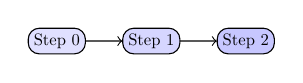
\begin{tikzpicture}[scale=0.6, transform shape]
  \node[draw,rounded corners,fill=blue!12] (n0) at (0.0,1) {Step 0};
  \node[draw,rounded corners,fill=blue!16] (n1) at (2.0,1) {Step 1};
  \node[draw,rounded corners,fill=blue!22] (n2) at (4.0,1) {Step 2};
  \draw[->] (n0) -- (n1);
  \draw[->] (n1) -- (n2);
\end{tikzpicture}
\end{center}
\end{frame}
\begin{frame}{Slide 12: synthetic topic}
\begin{itemize}
  \item \lipsum[13][1]
  \item \lipsum[14][2]
\end{itemize}
\begin{center}
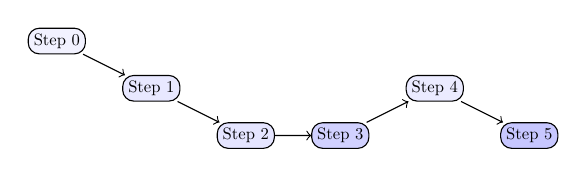
\begin{tikzpicture}[scale=0.6, transform shape]
  \node[draw,rounded corners,fill=blue!5] (n0) at (0.0,1) {Step 0};
  \node[draw,rounded corners,fill=blue!9] (n1) at (2.0,0) {Step 1};
  \node[draw,rounded corners,fill=blue!10] (n2) at (4.0,-1) {Step 2};
  \node[draw,rounded corners,fill=blue!18] (n3) at (6.0,-1) {Step 3};
  \node[draw,rounded corners,fill=blue!8] (n4) at (8.0,0) {Step 4};
  \node[draw,rounded corners,fill=blue!22] (n5) at (10.0,-1) {Step 5};
  \draw[->] (n0) -- (n1);
  \draw[->] (n1) -- (n2);
  \draw[->] (n2) -- (n3);
  \draw[->] (n3) -- (n4);
  \draw[->] (n4) -- (n5);
\end{tikzpicture}
\end{center}
\end{frame}
\begin{frame}{Slide 13: synthetic topic}
\begin{itemize}
  \item \lipsum[14][1]
  \item \lipsum[15][2]
\end{itemize}
\begin{center}
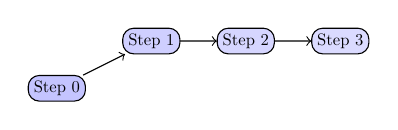
\begin{tikzpicture}[scale=0.6, transform shape]
  \node[draw,rounded corners,fill=blue!23] (n0) at (0.0,0) {Step 0};
  \node[draw,rounded corners,fill=blue!19] (n1) at (2.0,1) {Step 1};
  \node[draw,rounded corners,fill=blue!16] (n2) at (4.0,1) {Step 2};
  \node[draw,rounded corners,fill=blue!14] (n3) at (6.0,1) {Step 3};
  \draw[->] (n0) -- (n1);
  \draw[->] (n1) -- (n2);
  \draw[->] (n2) -- (n3);
\end{tikzpicture}
\end{center}
\end{frame}
\begin{frame}{Slide 14: synthetic topic}
\begin{itemize}
  \item \lipsum[15][1]
  \item \lipsum[16][2]
\end{itemize}
\begin{center}
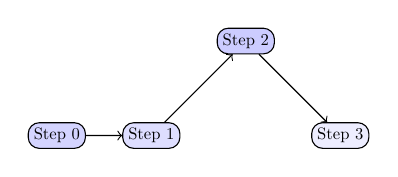
\begin{tikzpicture}[scale=0.6, transform shape]
  \node[draw,rounded corners,fill=blue!17] (n0) at (0.0,-1) {Step 0};
  \node[draw,rounded corners,fill=blue!13] (n1) at (2.0,-1) {Step 1};
  \node[draw,rounded corners,fill=blue!20] (n2) at (4.0,1) {Step 2};
  \node[draw,rounded corners,fill=blue!7] (n3) at (6.0,-1) {Step 3};
  \draw[->] (n0) -- (n1);
  \draw[->] (n1) -- (n2);
  \draw[->] (n2) -- (n3);
\end{tikzpicture}
\end{center}
\end{frame}
\begin{frame}{Slide 15: synthetic topic}
\begin{itemize}
  \item \lipsum[16][1]
  \item \lipsum[17][2]
\end{itemize}
\begin{center}
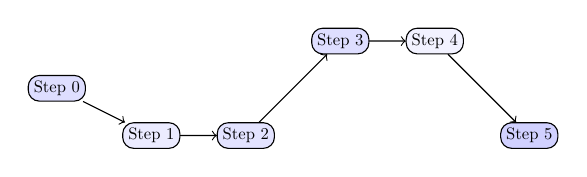
\begin{tikzpicture}[scale=0.6, transform shape]
  \node[draw,rounded corners,fill=blue!13] (n0) at (0.0,0) {Step 0};
  \node[draw,rounded corners,fill=blue!8] (n1) at (2.0,-1) {Step 1};
  \node[draw,rounded corners,fill=blue!11] (n2) at (4.0,-1) {Step 2};
  \node[draw,rounded corners,fill=blue!13] (n3) at (6.0,1) {Step 3};
  \node[draw,rounded corners,fill=blue!5] (n4) at (8.0,1) {Step 4};
  \node[draw,rounded corners,fill=blue!18] (n5) at (10.0,-1) {Step 5};
  \draw[->] (n0) -- (n1);
  \draw[->] (n1) -- (n2);
  \draw[->] (n2) -- (n3);
  \draw[->] (n3) -- (n4);
  \draw[->] (n4) -- (n5);
\end{tikzpicture}
\end{center}
\end{frame}
\begin{frame}{Slide 16: synthetic topic}
\begin{itemize}
  \item \lipsum[17][1]
  \item \lipsum[18][2]
\end{itemize}
\begin{center}
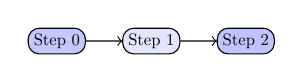
\begin{tikzpicture}[scale=0.6, transform shape]
  \node[draw,rounded corners,fill=blue!22] (n0) at (0.0,1) {Step 0};
  \node[draw,rounded corners,fill=blue!10] (n1) at (2.0,1) {Step 1};
  \node[draw,rounded corners,fill=blue!24] (n2) at (4.0,1) {Step 2};
  \draw[->] (n0) -- (n1);
  \draw[->] (n1) -- (n2);
\end{tikzpicture}
\end{center}
\end{frame}
\begin{frame}{Slide 17: synthetic topic}
\begin{itemize}
  \item \lipsum[18][1]
  \item \lipsum[19][2]
\end{itemize}
\begin{center}
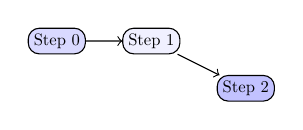
\begin{tikzpicture}[scale=0.6, transform shape]
  \node[draw,rounded corners,fill=blue!15] (n0) at (0.0,1) {Step 0};
  \node[draw,rounded corners,fill=blue!6] (n1) at (2.0,1) {Step 1};
  \node[draw,rounded corners,fill=blue!24] (n2) at (4.0,0) {Step 2};
  \draw[->] (n0) -- (n1);
  \draw[->] (n1) -- (n2);
\end{tikzpicture}
\end{center}
\end{frame}
\begin{frame}{Slide 18: synthetic topic}
\begin{itemize}
  \item \lipsum[19][1]
  \item \lipsum[20][2]
\end{itemize}
\begin{center}
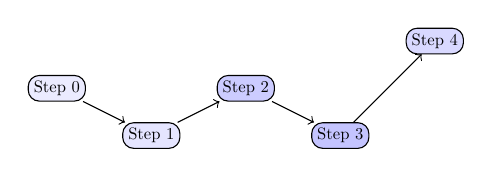
\begin{tikzpicture}[scale=0.6, transform shape]
  \node[draw,rounded corners,fill=blue!8] (n0) at (0.0,0) {Step 0};
  \node[draw,rounded corners,fill=blue!10] (n1) at (2.0,-1) {Step 1};
  \node[draw,rounded corners,fill=blue!20] (n2) at (4.0,0) {Step 2};
  \node[draw,rounded corners,fill=blue!23] (n3) at (6.0,-1) {Step 3};
  \node[draw,rounded corners,fill=blue!15] (n4) at (8.0,1) {Step 4};
  \draw[->] (n0) -- (n1);
  \draw[->] (n1) -- (n2);
  \draw[->] (n2) -- (n3);
  \draw[->] (n3) -- (n4);
\end{tikzpicture}
\end{center}
\end{frame}
\begin{frame}{Slide 19: synthetic topic}
\begin{itemize}
  \item \lipsum[20][1]
  \item \lipsum[21][2]
\end{itemize}
\begin{center}
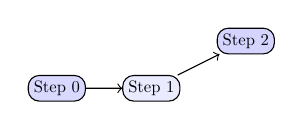
\begin{tikzpicture}[scale=0.6, transform shape]
  \node[draw,rounded corners,fill=blue!15] (n0) at (0.0,-1) {Step 0};
  \node[draw,rounded corners,fill=blue!8] (n1) at (2.0,-1) {Step 1};
  \node[draw,rounded corners,fill=blue!17] (n2) at (4.0,0) {Step 2};
  \draw[->] (n0) -- (n1);
  \draw[->] (n1) -- (n2);
\end{tikzpicture}
\end{center}
\end{frame}
\begin{frame}{Slide 20: synthetic topic}
\begin{itemize}
  \item \lipsum[1][1]
  \item \lipsum[2][2]
\end{itemize}
\begin{center}
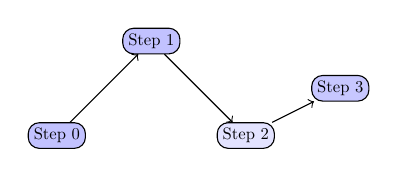
\begin{tikzpicture}[scale=0.6, transform shape]
  \node[draw,rounded corners,fill=blue!24] (n0) at (0.0,-1) {Step 0};
  \node[draw,rounded corners,fill=blue!24] (n1) at (2.0,1) {Step 1};
  \node[draw,rounded corners,fill=blue!11] (n2) at (4.0,-1) {Step 2};
  \node[draw,rounded corners,fill=blue!22] (n3) at (6.0,0) {Step 3};
  \draw[->] (n0) -- (n1);
  \draw[->] (n1) -- (n2);
  \draw[->] (n2) -- (n3);
\end{tikzpicture}
\end{center}
\end{frame}
\begin{frame}{Slide 21: synthetic topic}
\begin{itemize}
  \item \lipsum[2][1]
  \item \lipsum[3][2]
\end{itemize}
\begin{center}
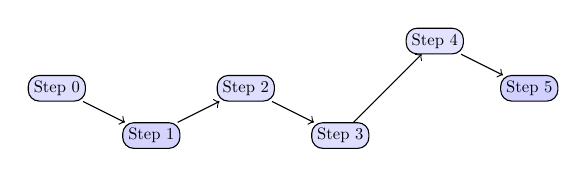
\begin{tikzpicture}[scale=0.6, transform shape]
  \node[draw,rounded corners,fill=blue!13] (n0) at (0.0,0) {Step 0};
  \node[draw,rounded corners,fill=blue!17] (n1) at (2.0,-1) {Step 1};
  \node[draw,rounded corners,fill=blue!13] (n2) at (4.0,0) {Step 2};
  \node[draw,rounded corners,fill=blue!13] (n3) at (6.0,-1) {Step 3};
  \node[draw,rounded corners,fill=blue!11] (n4) at (8.0,1) {Step 4};
  \node[draw,rounded corners,fill=blue!18] (n5) at (10.0,0) {Step 5};
  \draw[->] (n0) -- (n1);
  \draw[->] (n1) -- (n2);
  \draw[->] (n2) -- (n3);
  \draw[->] (n3) -- (n4);
  \draw[->] (n4) -- (n5);
\end{tikzpicture}
\end{center}
\end{frame}
\begin{frame}{Slide 22: synthetic topic}
\begin{itemize}
  \item \lipsum[3][1]
  \item \lipsum[4][2]
\end{itemize}
\begin{center}
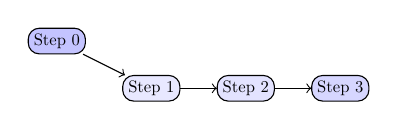
\begin{tikzpicture}[scale=0.6, transform shape]
  \node[draw,rounded corners,fill=blue!23] (n0) at (0.0,1) {Step 0};
  \node[draw,rounded corners,fill=blue!9] (n1) at (2.0,0) {Step 1};
  \node[draw,rounded corners,fill=blue!11] (n2) at (4.0,0) {Step 2};
  \node[draw,rounded corners,fill=blue!16] (n3) at (6.0,0) {Step 3};
  \draw[->] (n0) -- (n1);
  \draw[->] (n1) -- (n2);
  \draw[->] (n2) -- (n3);
\end{tikzpicture}
\end{center}
\end{frame}
\begin{frame}{Slide 23: synthetic topic}
\begin{itemize}
  \item \lipsum[4][1]
  \item \lipsum[5][2]
\end{itemize}
\begin{center}
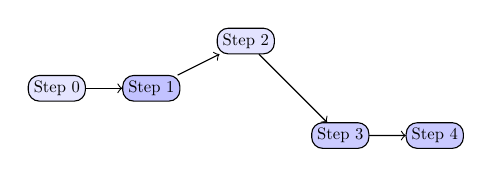
\begin{tikzpicture}[scale=0.6, transform shape]
  \node[draw,rounded corners,fill=blue!10] (n0) at (0.0,0) {Step 0};
  \node[draw,rounded corners,fill=blue!24] (n1) at (2.0,0) {Step 1};
  \node[draw,rounded corners,fill=blue!11] (n2) at (4.0,1) {Step 2};
  \node[draw,rounded corners,fill=blue!20] (n3) at (6.0,-1) {Step 3};
  \node[draw,rounded corners,fill=blue!21] (n4) at (8.0,-1) {Step 4};
  \draw[->] (n0) -- (n1);
  \draw[->] (n1) -- (n2);
  \draw[->] (n2) -- (n3);
  \draw[->] (n3) -- (n4);
\end{tikzpicture}
\end{center}
\end{frame}
\begin{frame}{Slide 24: synthetic topic}
\begin{itemize}
  \item \lipsum[5][1]
  \item \lipsum[6][2]
\end{itemize}
\begin{center}
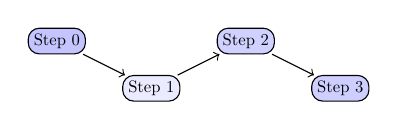
\begin{tikzpicture}[scale=0.6, transform shape]
  \node[draw,rounded corners,fill=blue!23] (n0) at (0.0,1) {Step 0};
  \node[draw,rounded corners,fill=blue!8] (n1) at (2.0,0) {Step 1};
  \node[draw,rounded corners,fill=blue!18] (n2) at (4.0,1) {Step 2};
  \node[draw,rounded corners,fill=blue!19] (n3) at (6.0,0) {Step 3};
  \draw[->] (n0) -- (n1);
  \draw[->] (n1) -- (n2);
  \draw[->] (n2) -- (n3);
\end{tikzpicture}
\end{center}
\end{frame}
\begin{frame}{Slide 25: synthetic topic}
\begin{itemize}
  \item \lipsum[6][1]
  \item \lipsum[7][2]
\end{itemize}
\begin{center}
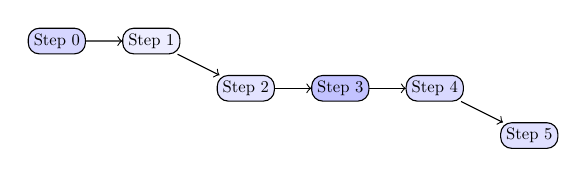
\begin{tikzpicture}[scale=0.6, transform shape]
  \node[draw,rounded corners,fill=blue!16] (n0) at (0.0,1) {Step 0};
  \node[draw,rounded corners,fill=blue!7] (n1) at (2.0,1) {Step 1};
  \node[draw,rounded corners,fill=blue!11] (n2) at (4.0,0) {Step 2};
  \node[draw,rounded corners,fill=blue!24] (n3) at (6.0,0) {Step 3};
  \node[draw,rounded corners,fill=blue!15] (n4) at (8.0,0) {Step 4};
  \node[draw,rounded corners,fill=blue!12] (n5) at (10.0,-1) {Step 5};
  \draw[->] (n0) -- (n1);
  \draw[->] (n1) -- (n2);
  \draw[->] (n2) -- (n3);
  \draw[->] (n3) -- (n4);
  \draw[->] (n4) -- (n5);
\end{tikzpicture}
\end{center}
\end{frame}
\begin{frame}{Slide 26: synthetic topic}
\begin{itemize}
  \item \lipsum[7][1]
  \item \lipsum[8][2]
\end{itemize}
\begin{center}
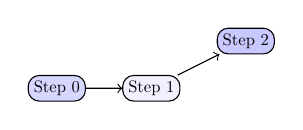
\begin{tikzpicture}[scale=0.6, transform shape]
  \node[draw,rounded corners,fill=blue!16] (n0) at (0.0,-1) {Step 0};
  \node[draw,rounded corners,fill=blue!6] (n1) at (2.0,-1) {Step 1};
  \node[draw,rounded corners,fill=blue!21] (n2) at (4.0,0) {Step 2};
  \draw[->] (n0) -- (n1);
  \draw[->] (n1) -- (n2);
\end{tikzpicture}
\end{center}
\end{frame}
\begin{frame}{Slide 27: synthetic topic}
\begin{itemize}
  \item \lipsum[8][1]
  \item \lipsum[9][2]
\end{itemize}
\begin{center}
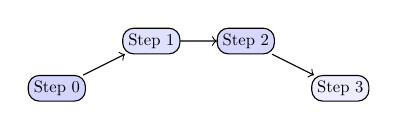
\begin{tikzpicture}[scale=0.6, transform shape]
  \node[draw,rounded corners,fill=blue!17] (n0) at (0.0,0) {Step 0};
  \node[draw,rounded corners,fill=blue!12] (n1) at (2.0,1) {Step 1};
  \node[draw,rounded corners,fill=blue!16] (n2) at (4.0,1) {Step 2};
  \node[draw,rounded corners,fill=blue!7] (n3) at (6.0,0) {Step 3};
  \draw[->] (n0) -- (n1);
  \draw[->] (n1) -- (n2);
  \draw[->] (n2) -- (n3);
\end{tikzpicture}
\end{center}
\end{frame}
\begin{frame}{Slide 28: synthetic topic}
\begin{itemize}
  \item \lipsum[9][1]
  \item \lipsum[10][2]
\end{itemize}
\begin{center}
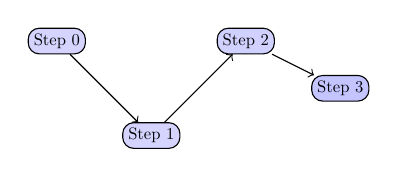
\begin{tikzpicture}[scale=0.6, transform shape]
  \node[draw,rounded corners,fill=blue!17] (n0) at (0.0,1) {Step 0};
  \node[draw,rounded corners,fill=blue!17] (n1) at (2.0,-1) {Step 1};
  \node[draw,rounded corners,fill=blue!18] (n2) at (4.0,1) {Step 2};
  \node[draw,rounded corners,fill=blue!23] (n3) at (6.0,0) {Step 3};
  \draw[->] (n0) -- (n1);
  \draw[->] (n1) -- (n2);
  \draw[->] (n2) -- (n3);
\end{tikzpicture}
\end{center}
\end{frame}
\begin{frame}{Slide 29: synthetic topic}
\begin{itemize}
  \item \lipsum[10][1]
  \item \lipsum[11][2]
\end{itemize}
\begin{center}
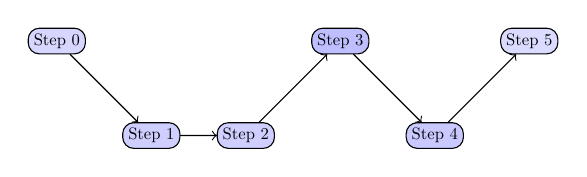
\begin{tikzpicture}[scale=0.6, transform shape]
  \node[draw,rounded corners,fill=blue!16] (n0) at (0.0,1) {Step 0};
  \node[draw,rounded corners,fill=blue!19] (n1) at (2.0,-1) {Step 1};
  \node[draw,rounded corners,fill=blue!19] (n2) at (4.0,-1) {Step 2};
  \node[draw,rounded corners,fill=blue!25] (n3) at (6.0,1) {Step 3};
  \node[draw,rounded corners,fill=blue!21] (n4) at (8.0,-1) {Step 4};
  \node[draw,rounded corners,fill=blue!14] (n5) at (10.0,1) {Step 5};
  \draw[->] (n0) -- (n1);
  \draw[->] (n1) -- (n2);
  \draw[->] (n2) -- (n3);
  \draw[->] (n3) -- (n4);
  \draw[->] (n4) -- (n5);
\end{tikzpicture}
\end{center}
\end{frame}
\begin{frame}{Slide 30: synthetic topic}
\begin{itemize}
  \item \lipsum[11][1]
  \item \lipsum[12][2]
\end{itemize}
\begin{center}
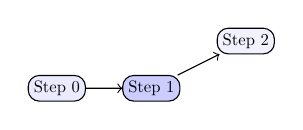
\begin{tikzpicture}[scale=0.6, transform shape]
  \node[draw,rounded corners,fill=blue!8] (n0) at (0.0,-1) {Step 0};
  \node[draw,rounded corners,fill=blue!20] (n1) at (2.0,-1) {Step 1};
  \node[draw,rounded corners,fill=blue!5] (n2) at (4.0,0) {Step 2};
  \draw[->] (n0) -- (n1);
  \draw[->] (n1) -- (n2);
\end{tikzpicture}
\end{center}
\end{frame}
\begin{frame}{Slide 31: synthetic topic}
\begin{itemize}
  \item \lipsum[12][1]
  \item \lipsum[13][2]
\end{itemize}
\begin{center}
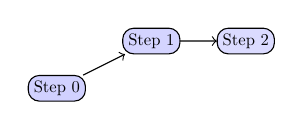
\begin{tikzpicture}[scale=0.6, transform shape]
  \node[draw,rounded corners,fill=blue!18] (n0) at (0.0,0) {Step 0};
  \node[draw,rounded corners,fill=blue!17] (n1) at (2.0,1) {Step 1};
  \node[draw,rounded corners,fill=blue!14] (n2) at (4.0,1) {Step 2};
  \draw[->] (n0) -- (n1);
  \draw[->] (n1) -- (n2);
\end{tikzpicture}
\end{center}
\end{frame}
\begin{frame}{Slide 32: synthetic topic}
\begin{itemize}
  \item \lipsum[13][1]
  \item \lipsum[14][2]
\end{itemize}
\begin{center}
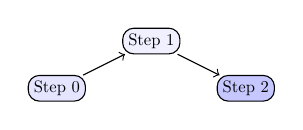
\begin{tikzpicture}[scale=0.6, transform shape]
  \node[draw,rounded corners,fill=blue!10] (n0) at (0.0,-1) {Step 0};
  \node[draw,rounded corners,fill=blue!6] (n1) at (2.0,0) {Step 1};
  \node[draw,rounded corners,fill=blue!22] (n2) at (4.0,-1) {Step 2};
  \draw[->] (n0) -- (n1);
  \draw[->] (n1) -- (n2);
\end{tikzpicture}
\end{center}
\end{frame}
\begin{frame}{Slide 33: synthetic topic}
\begin{itemize}
  \item \lipsum[14][1]
  \item \lipsum[15][2]
\end{itemize}
\begin{center}
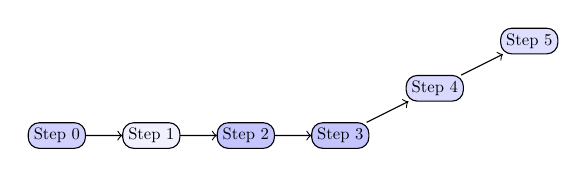
\begin{tikzpicture}[scale=0.6, transform shape]
  \node[draw,rounded corners,fill=blue!18] (n0) at (0.0,-1) {Step 0};
  \node[draw,rounded corners,fill=blue!6] (n1) at (2.0,-1) {Step 1};
  \node[draw,rounded corners,fill=blue!23] (n2) at (4.0,-1) {Step 2};
  \node[draw,rounded corners,fill=blue!23] (n3) at (6.0,-1) {Step 3};
  \node[draw,rounded corners,fill=blue!15] (n4) at (8.0,0) {Step 4};
  \node[draw,rounded corners,fill=blue!13] (n5) at (10.0,1) {Step 5};
  \draw[->] (n0) -- (n1);
  \draw[->] (n1) -- (n2);
  \draw[->] (n2) -- (n3);
  \draw[->] (n3) -- (n4);
  \draw[->] (n4) -- (n5);
\end{tikzpicture}
\end{center}
\end{frame}
\begin{frame}{Slide 34: synthetic topic}
\begin{itemize}
  \item \lipsum[15][1]
  \item \lipsum[16][2]
\end{itemize}
\begin{center}
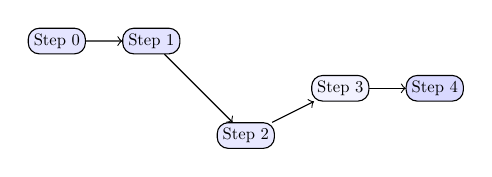
\begin{tikzpicture}[scale=0.6, transform shape]
  \node[draw,rounded corners,fill=blue!10] (n0) at (0.0,1) {Step 0};
  \node[draw,rounded corners,fill=blue!11] (n1) at (2.0,1) {Step 1};
  \node[draw,rounded corners,fill=blue!9] (n2) at (4.0,-1) {Step 2};
  \node[draw,rounded corners,fill=blue!5] (n3) at (6.0,0) {Step 3};
  \node[draw,rounded corners,fill=blue!15] (n4) at (8.0,0) {Step 4};
  \draw[->] (n0) -- (n1);
  \draw[->] (n1) -- (n2);
  \draw[->] (n2) -- (n3);
  \draw[->] (n3) -- (n4);
\end{tikzpicture}
\end{center}
\end{frame}
\begin{frame}{Slide 35: synthetic topic}
\begin{itemize}
  \item \lipsum[16][1]
  \item \lipsum[17][2]
\end{itemize}
\begin{center}
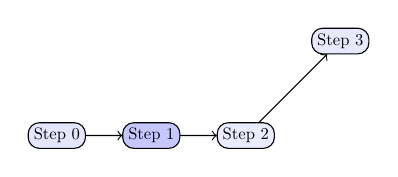
\begin{tikzpicture}[scale=0.6, transform shape]
  \node[draw,rounded corners,fill=blue!10] (n0) at (0.0,-1) {Step 0};
  \node[draw,rounded corners,fill=blue!22] (n1) at (2.0,-1) {Step 1};
  \node[draw,rounded corners,fill=blue!8] (n2) at (4.0,-1) {Step 2};
  \node[draw,rounded corners,fill=blue!9] (n3) at (6.0,1) {Step 3};
  \draw[->] (n0) -- (n1);
  \draw[->] (n1) -- (n2);
  \draw[->] (n2) -- (n3);
\end{tikzpicture}
\end{center}
\end{frame}
\begin{frame}{Slide 36: synthetic topic}
\begin{itemize}
  \item \lipsum[17][1]
  \item \lipsum[18][2]
\end{itemize}
\begin{center}
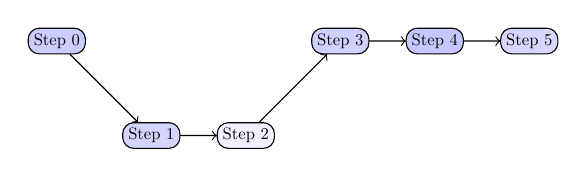
\begin{tikzpicture}[scale=0.6, transform shape]
  \node[draw,rounded corners,fill=blue!20] (n0) at (0.0,1) {Step 0};
  \node[draw,rounded corners,fill=blue!17] (n1) at (2.0,-1) {Step 1};
  \node[draw,rounded corners,fill=blue!6] (n2) at (4.0,-1) {Step 2};
  \node[draw,rounded corners,fill=blue!18] (n3) at (6.0,1) {Step 3};
  \node[draw,rounded corners,fill=blue!22] (n4) at (8.0,1) {Step 4};
  \node[draw,rounded corners,fill=blue!16] (n5) at (10.0,1) {Step 5};
  \draw[->] (n0) -- (n1);
  \draw[->] (n1) -- (n2);
  \draw[->] (n2) -- (n3);
  \draw[->] (n3) -- (n4);
  \draw[->] (n4) -- (n5);
\end{tikzpicture}
\end{center}
\end{frame}
\begin{frame}{Slide 37: synthetic topic}
\begin{itemize}
  \item \lipsum[18][1]
  \item \lipsum[19][2]
\end{itemize}
\begin{center}
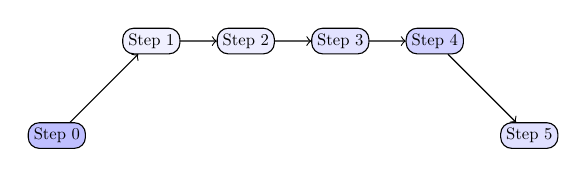
\begin{tikzpicture}[scale=0.6, transform shape]
  \node[draw,rounded corners,fill=blue!25] (n0) at (0.0,-1) {Step 0};
  \node[draw,rounded corners,fill=blue!6] (n1) at (2.0,1) {Step 1};
  \node[draw,rounded corners,fill=blue!7] (n2) at (4.0,1) {Step 2};
  \node[draw,rounded corners,fill=blue!11] (n3) at (6.0,1) {Step 3};
  \node[draw,rounded corners,fill=blue!18] (n4) at (8.0,1) {Step 4};
  \node[draw,rounded corners,fill=blue!12] (n5) at (10.0,-1) {Step 5};
  \draw[->] (n0) -- (n1);
  \draw[->] (n1) -- (n2);
  \draw[->] (n2) -- (n3);
  \draw[->] (n3) -- (n4);
  \draw[->] (n4) -- (n5);
\end{tikzpicture}
\end{center}
\end{frame}
\begin{frame}{Slide 38: synthetic topic}
\begin{itemize}
  \item \lipsum[19][1]
  \item \lipsum[20][2]
\end{itemize}
\begin{center}
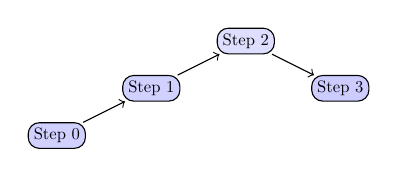
\begin{tikzpicture}[scale=0.6, transform shape]
  \node[draw,rounded corners,fill=blue!18] (n0) at (0.0,-1) {Step 0};
  \node[draw,rounded corners,fill=blue!18] (n1) at (2.0,0) {Step 1};
  \node[draw,rounded corners,fill=blue!13] (n2) at (4.0,1) {Step 2};
  \node[draw,rounded corners,fill=blue!20] (n3) at (6.0,0) {Step 3};
  \draw[->] (n0) -- (n1);
  \draw[->] (n1) -- (n2);
  \draw[->] (n2) -- (n3);
\end{tikzpicture}
\end{center}
\end{frame}
\begin{frame}{Slide 39: synthetic topic}
\begin{itemize}
  \item \lipsum[20][1]
  \item \lipsum[21][2]
\end{itemize}
\begin{center}
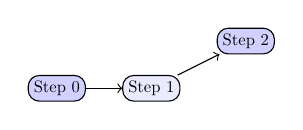
\begin{tikzpicture}[scale=0.6, transform shape]
  \node[draw,rounded corners,fill=blue!18] (n0) at (0.0,0) {Step 0};
  \node[draw,rounded corners,fill=blue!8] (n1) at (2.0,0) {Step 1};
  \node[draw,rounded corners,fill=blue!18] (n2) at (4.0,1) {Step 2};
  \draw[->] (n0) -- (n1);
  \draw[->] (n1) -- (n2);
\end{tikzpicture}
\end{center}
\end{frame}
\begin{frame}{Slide 40: synthetic topic}
\begin{itemize}
  \item \lipsum[1][1]
  \item \lipsum[2][2]
\end{itemize}
\begin{center}
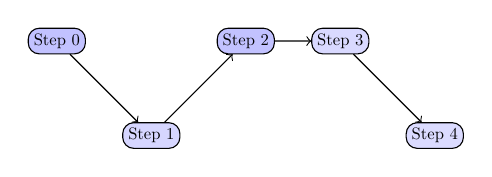
\begin{tikzpicture}[scale=0.6, transform shape]
  \node[draw,rounded corners,fill=blue!24] (n0) at (0.0,1) {Step 0};
  \node[draw,rounded corners,fill=blue!16] (n1) at (2.0,-1) {Step 1};
  \node[draw,rounded corners,fill=blue!24] (n2) at (4.0,1) {Step 2};
  \node[draw,rounded corners,fill=blue!15] (n3) at (6.0,1) {Step 3};
  \node[draw,rounded corners,fill=blue!14] (n4) at (8.0,-1) {Step 4};
  \draw[->] (n0) -- (n1);
  \draw[->] (n1) -- (n2);
  \draw[->] (n2) -- (n3);
  \draw[->] (n3) -- (n4);
\end{tikzpicture}
\end{center}
\end{frame}
\end{document}
